\chapter{Riemann Pump circuit design}
\label{ch:design}
% \textit{Description of the approach you have taken to solve the scientific or technical problem which you were posed. Outline the design, the methodology and overall structure of your experimental approach}\\
The goal was to design an arbitrary waveform generator for a signal bandwidth of \SI{6}{\giga \hertz}.
For the implementation in a base station, the most promising technology was \gls{ab:gan}.
\gls{ab:gan} \glspl{ab:hemt} were used for the high speed switches, which served as voltage controlled current sources.
Based on the chosen technology a suitable push-pull concept were found \cite{MaksimovicPaper} to show the feasibility of the concept.
The attention was rather drawn to proof the concept than to optimize for energy consumption or efficiency.
In the design process a suitable load impedance and the right dimension of the used components had to be found.

\section{Approach and implementation of the Riemann Pump}
As stated in chapter \ref{IdeaRiemannPump} the circuit needed high speed switches, which were capable to drive power.
The absence of a p-type transistor in \gls{ab:gan} technology made it challenging to find a suitable concept to realize the push-pull stage.
Since the n-type \glspl{ab:hemt} needed a negative gate source voltage \gls{sy:vgs}, the high side switch could not be implemented without a driver circuit.
The source contact of the high side switch, realized by a n-type \gls{ab:gan} \gls{ab:hemt}, was connected to the output of the test circuit.
Since the potential at the output was not constant, this high side switch needed a driver circuit.
A suitable driver circuit was found in \cite{MaksimovicPaper}, where the principle of a push-pull stage for power applications is described.
The benefit of the integrated driver circuit was the improved efficiency of switching.
The transistor switching speed was determined by the dimension of the driver circuit.
If the switching speed was increased, the gate driving current \gls{sy:IG} has to be increased to switch the transistors.\\
One possible approach to design a Riemann Pump is shown in Fig. \ref{fig:SchematicRiemannPump}.

\begin{figure}[ht]
	\centering
  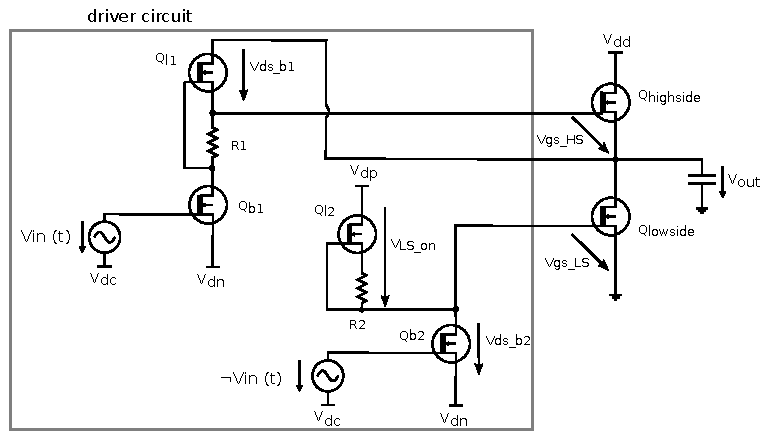
\includegraphics{Schematic_RP_concept2.pdf}
	\caption{Schematic of a push-pull stage with corresponding driver circuit}
	\label{fig:SchematicRiemannPump}
\end{figure}

%%%%%%%%%%%%%%% 00:40 Uhr 01.05.2016
On the left side, as marked, is the driver circuit which was needed to switch the high side transistor without dissipating a huge amount of power.
As the timing is crucial for the switching process, the driver concept was implemented for the low side switch too.
Each driver consisted of a base transistor, marked as Qb1 and Qb2, which served to operate as a inverter.
If the this base transistor is switched on, the potential \gls{sy:vdn} is fed to the resistor and hence to the power transistor. 
Two power transistors were designed and were marked as Qhighside and Qlowside, since they switch the output either to the high side power rail or to the low side power rail.
Once the potential of \gls{sy:vdn} is fed to the power transistor, this transistor is switched off, hence it became a inverter structure.

The schematic shows the first approach for realizing a Riemann Pump in \gls{ab:gan} technology.
The next step was the identification and calculation of a proper output capacitance, since it represented the input of a linear power amplifier where the desired signal is synthesized.
 
\section{Identification of the load impedance} % VERBESSERN!
The signal is generated at the input stage of a linear power amplifier, as described in chapter \ref{ch:fundamentals}.
This output stage is modelled with a \gls{ab:gan} \gls{ab:hemt} with a gate length of \SI{0.25}{\micro \meter}.
Considering a \SI{20}{\watt} power amplifier for transmission purposes, led to a \gls{ab:gan} \gls{ab:hemt} with a total gate periphery of \SI{4}{\milli \metre}, based on an approximation for the power density of \SI[per-mode=fraction]{5}{\watt\per\milli\metre} gate periphery  \cite{Maroldt2010}, \cite{GaNBook}.
Simulations confirmed this approximation as an output power density of \SI[per-mode=fraction]{5.6}{\watt\per\milli\metre} at $V_{DS} = 25 V$ was measured.
This transistor model \gls{ab:hemt} (IAF\_GE\_MSL\_ A204/IAF\_GaN25\_HEMT\_CS\_LS\_SHfull) used in \gls{ab:ads} were modelled at the \gls{ab:iaf}\cite{model} and is based on a state-space approach. 
For simulation purposes four transistors were modelled in parallel, each with 8 finger and \SI{125}{\micro \metre} gate width to reach the required gate periphery.
The simulated power amplifier is biased with respect to the maximum \gls{ab:mag}, which led to a bias of $V_{GS} = -1.5 V$ at $V_{DS} = 25 V$.
After the determination of the bias point, a S-parameter simulation yielded the input reactance of the power amplifier.
It is to note that four power transistors were simulated for the purpose of a power amplifier, hence this did not respect the broadband application since it was no broadband amplifier.
Since the capacitive behaviour of the load impedance is of interest, the real part is for now neglected.
The input reactance $X_c$ is defined as:
\begin{equation}
	X_c = -\frac{1}{\omega C},
\end{equation}
\label{eq:reactance}
and is plotted in Figure \ref{fig:inputReactance} over the frequency range from nearly \gls{ab:dc} to \SI{6}{\giga \hertz} in a logarithmic scale.

\begin{figure}[ht]
	\centering
  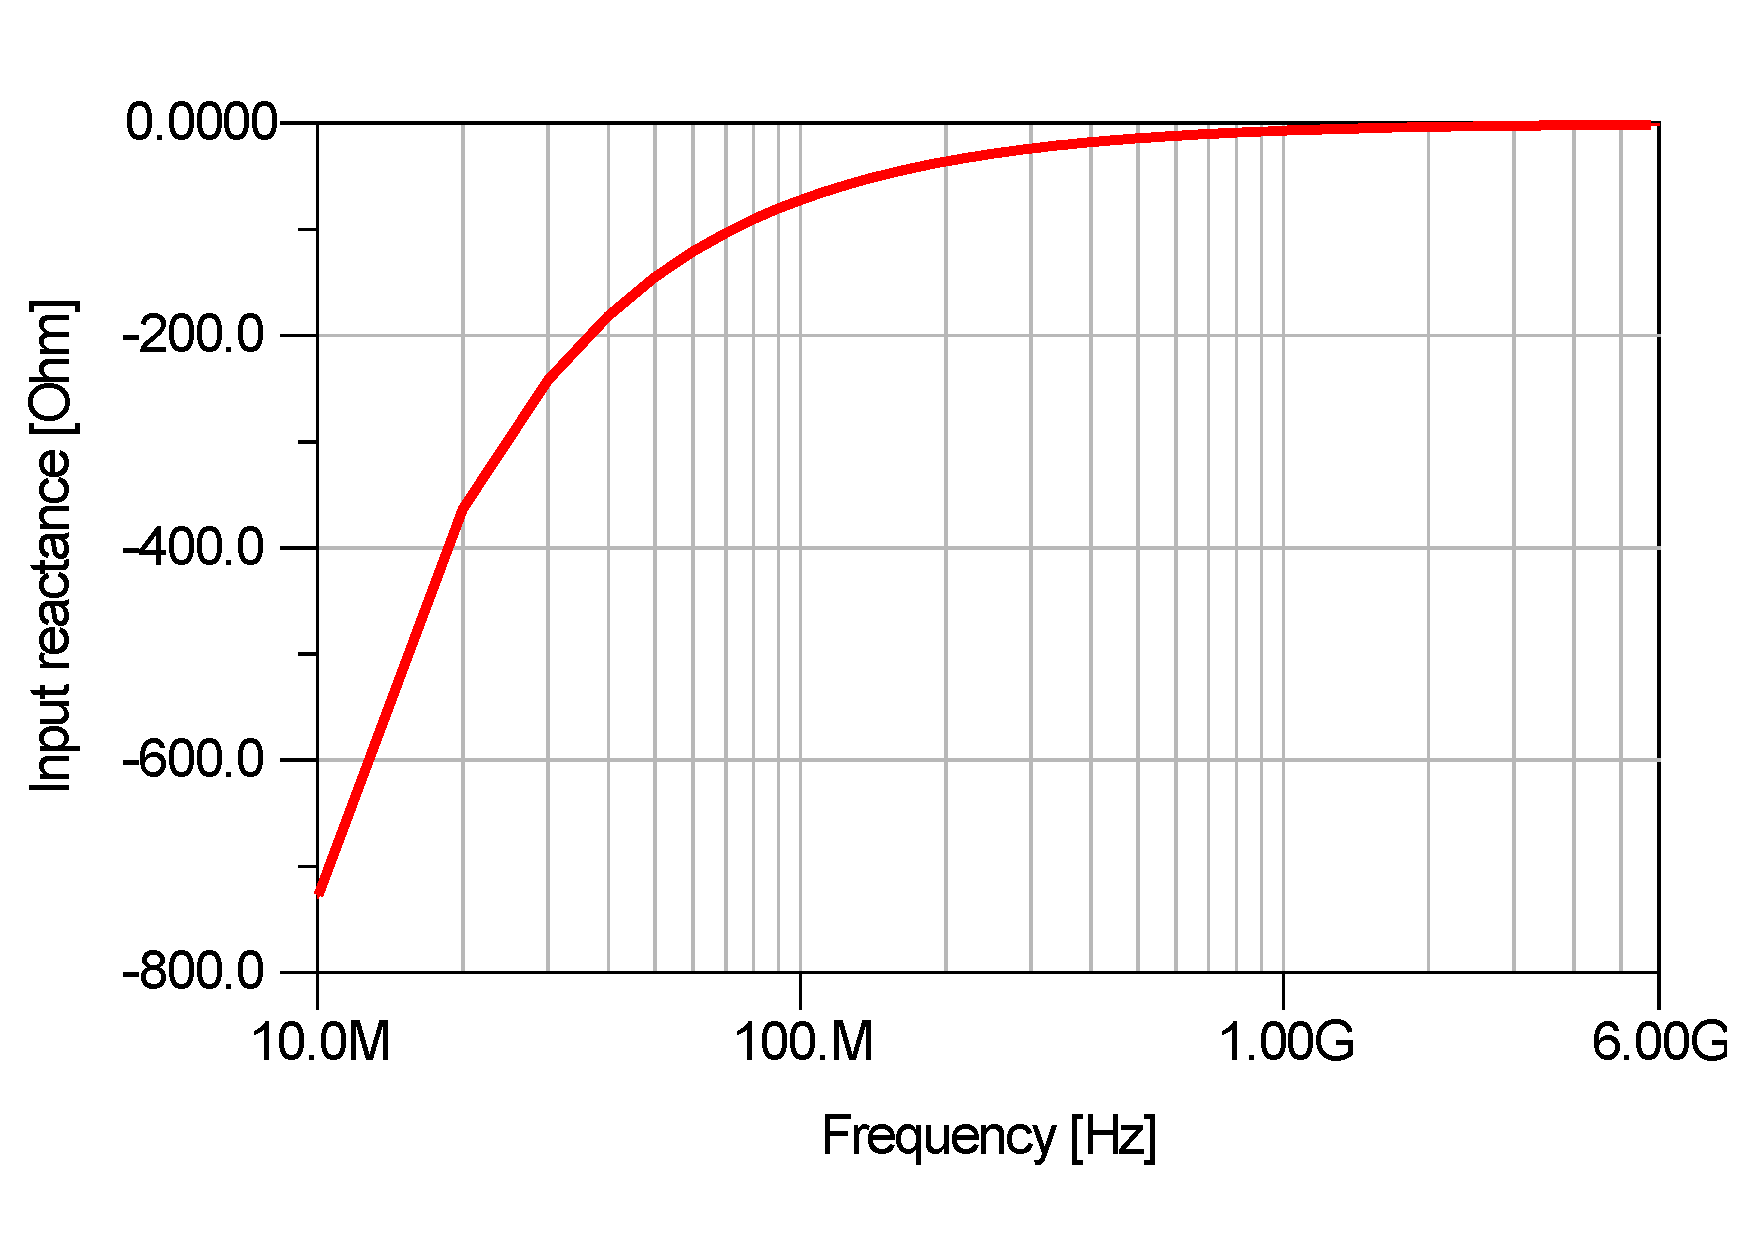
\includegraphics[width=.75\textwidth]{inputReactance.pdf}
	\caption{load reactance}
	\label{fig:inputReactance}
\end{figure}

As the reactance of the simulated power amplifier is nearly constant for the frequency of \SI{1}{\giga \hertz} and beyond, this showed the impact of parasitic effects.
For frequencies in the \si{\giga \hertz} range the parasitic inductances reduced the reactance.
Interpreting the minus sign only for the phase delay, since it is capacitive, the absolute value of the reactance decreases exponentially with the frequency up to approximately \SI{1}{\giga \hertz}.
Solving the equations \ref{eq:reactance} absolute value for the capacitance yielded:

\begin{equation}
	C = \frac{1}{\omega X_c},
\end{equation}
which is illustrated in Figure \ref{fig:inputCap_log}.
As a large signal model was used for the simulation, the inductive part of the input impedance got bigger.
This effect is seen in \ref{fig:inputCap_log} for frequencies beyond \SI{1}{\giga \hertz}.
%The frequency dispersion effect on the input capacitance of the \gls{ab:gan} \gls{ab:hemt}
\begin{figure}[ht]
	\centering
  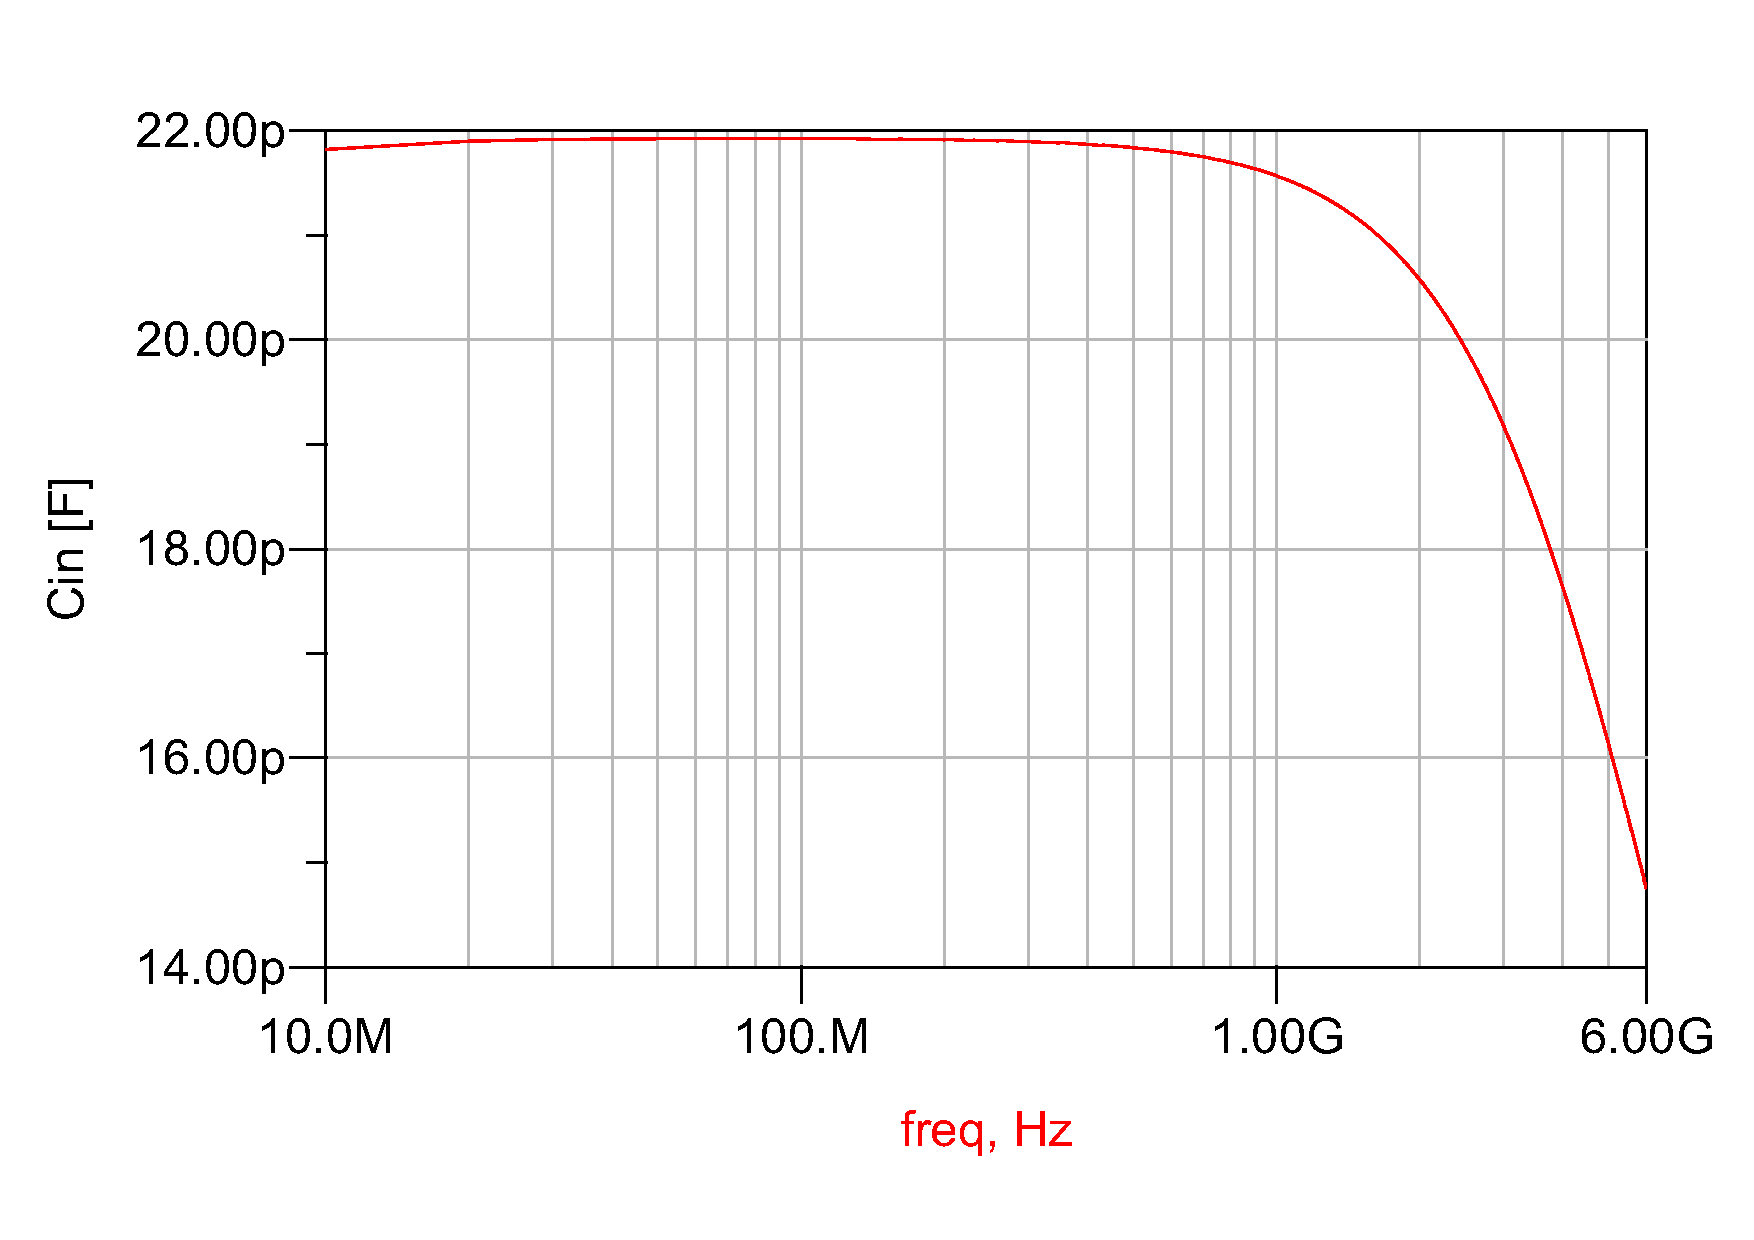
\includegraphics[width=.75\textwidth]{inputCap_log.pdf}
	\caption{load capacitance log}
	\label{fig:inputCap_log}
\end{figure}

Nevertheless the complex input impedance yielded a capacitive behaviour with a value of nearly \SI{22}{\pico \farad}, which was used for further investigations.
The simulated transistor model was specified as a large signal model, as seen in Figure \ref{fig:inputCap_log} for frequencies beyond \SI{1}{\giga \hertz}.
Frequency dispersion and other parasitic effects appeared, which could not be investigated due to the limited scope of this thesis.

%
%Since the input capacitance can be assumed as 
%\begin{equation}
%	C = \epsilon_r \frac{A}{d},
%\end{equation}
%
%it follows that
%\begin{equation}
%	C \propto \epsilon_r 
%\end{equation}
%
%and therefore for high frequencies, the capacitance is decreasing due to decreasing dielectric constant for \gls{ab:gan} \cite{GaNBook},p.7. % pdf page 33
%Degrading capacitance due to non-linearities.

%Due to the non-linearity of the transistor model \cite{vitanovnon}
%The frequency dependent input impedance [\textbf{REFERENCE}], which corresponds to the load impedance of the designed Riemann pump circuit, is determined by S-parameter simulations.
% small signal is not considered, since only the curent integration is important

%%% 27.04.2016 01:34 Uhr
\section{Dimension of the used components}
An input capacitance of nearly \SI{22}{\pico \farad} was found for the output linear power amplifier stage.
Based on this calculation a proper test circuit was investigated.
To avoid immediate clipping of the signal at the output, the transistor dimension had to fit, since an oversized transistor would fully charge the capacitance and the signal would be clipped.
Hence a transistor dimension was chosen which allowed to synthesize a decent signal.
To synthesize a sine wave for the frequency of \SI{6}{\giga \hertz} with a voltage swing of $V_{swing} = 4V$, the two greatest slopes were chosen.
In the presented concept the resolution is three bit, hence eight different current slopes could be generated.
The sequence of the relative slopes $7 i_0$ and $5 i_0$ synthesize the rising edge of the sine wave.
With this relative slopes and an oversampling ratio of four at the frequency of \SI{6}{\giga \hertz}, led to a sampling time $\Delta t$ of \SI{20.83}{\pico \second}, since the sampling frequency is eight times the signal bandwidth.

The current-voltage relation for the capacitor
\begin{equation}
	I = C \frac{d U}{d t},
\end{equation}
is used to determine the reference current $i_0$.

A voltage swing of $V_{swing} = 4V$ is equal to an amplitude of $\hat{v} = 2V$.
The oversampling of four yielded, that the sine signal is sampled by eight points.
Hence the rising edge consisted of two sampling points.
The first sampling point with the relative slope of 7 and the second of 5, respectively.
Integrating the current for two different samples yield:

\begin{equation}
\int_{\Delta t} 7 i_0 d\tau + \int_{\Delta t} 5 i_0 d \tau = C*U,
\end{equation}

and solving for $i_0$ resulted in:

\begin{equation}
i_0 = \frac{U*C}{12*\Delta t}.
\end{equation}

For the assumption to reach nearly a voltage of $\hat{v} = 2V$ for two sampling intervals ($2 \Delta t$) and the capacitance of \SI{20}{\pico \farad} it resulted a reference current of $i_0 = \SI{160}{\milli \ampere}$.
%The dimension of the switching transistors, which represent a voltage controlled current source, determines the maximum current flowing.
%This current source is controlled by a digital signal which determines it to be fully open or to be closed, as a switch.
As simulations showed, a reference current of $\SI{151}{\milli \ampere}$ could be established with a dimension of the voltage controlled current source, high side switch, of UGW = 100 \si{\micro \meter} and gate finger number of eight.
Hence the gate periphery for the reference current source is \SI{800}{\micro \meter}.
To ensure proper switching the driver circuit dimension had to be optimized.
Since the driver circuit worked as a current source, the dimension of the transistors and resistors were tuned to achieve a proper current to switch the power transistors fast and efficient.
The dimension of the driver transistors were approximately a quarter of the power transistors, the switching high and low side transistor.
The resistor values were achieved by tuning with respect to power consumption.
Further details on the driver circuit and its properties are stated in \cite{MaksimovicPaper}.
The schematic is designed with \gls{ab:ads}, see Appendix \ref{app:schematic}.
As the dimension of the power stage scales with the factor of two so the driver circuit dimension do.

\section{Circuit design summary}
As no complementary transistors were available in III-V technology a proper driver circuit had to be investigated.
Further the speed of the switches was crucial as a broadband signal should be synthesized, which led to the implementation of a known concept \cite{MaksimovicPaper} for the driver circuit.
A low loss, high speed, digital controlled driver circuit was implemented.
Using this concept had the advantage of verification and validation.
It was difficult to determine the reference current since the switching is not ideal, a leakage current through the driver circuit occurs and the current had to be probed in the transient state.
The problem of not perfect switching is, that the channel is opened and closed slowly in comparison to an ideal switch.
This increase the current with the increase of charges flowing to the transistors gate.
Therefore the reference current is time-averaged.
The circuit design and simulation combines the dc state with the rf state.
For a dc simulation the current through a capacitor is zero.
Further the loaded voltage controlled current source was not defined for the given output load.
The dimension of the used components determined the resulting voltage step.
A typical (draw-back) contradiction was a small transistor dimension could synthesize signals to a very low signal frequency while a bigger one would fully charge the output capacitor which will clip the output signal, for a given oversampling ratio.
Because then the sampling time is fixed.
If the transistor dimension is chosen to be bigger, the higher signal frequency could be synthesized with a decent voltage swing but the low signal frequencies would turn into a rectangular shape. 
This problem restricted the signal bandwidth to be smaller than from \gls{ab:dc} to \SI{6}{\GHz}.

%  The components used, were optimized with respect to the signal integrity. 
%  The dimension of the used components were tuned while simulation to get the desired output signal.
%In contrast to the small one a bigger one will be able to synthesize a signal at 6GHz due to the fact that the amplitude would be moderate.

%The smallest current is determined by the dimension of the transistor, which drives into saturation. 
%The smallest saturated current is determined by the push-pull transistor geometry, here: 532 mA.}